\documentclass{article}
\usepackage{graphicx}
\usepackage{array}
\begin{document}

% --- TITLE PAGE --- %

\begin{titlepage}
\newcommand{\HRule}{\rule{\linewidth}{0.5mm}}
\center
\textsc{\LARGE Imperial College London}  \\[1.5cm]
\textsc{\Large Department of Computing}  \\[0.5cm]
\textsc{\large Course 350: Management and Business for Computing Engineers} \\[0.5cm]

\HRule \\[0.6cm]
{\huge \bfseries SubZero Ice} \\[0.3cm]
\HRule \\[1.5cm]

\begin{minipage}{0.4\textwidth}

% author
\begin{flushleft} \large \emph{Authors:} \\
Tim       \textsc{Gates}   \\
Ben       \textsc{Homer}   \\
Graham    \textsc{Lyon}    \\
Conor     \textsc{Nevin}   \\
Martin    \textsc{Sidery}  \\
Jon       \textsc{Watson}  \\
\end{flushleft}

% lecturer
\end{minipage}~
\begin{minipage}{0.4\textwidth}

\begin{flushright} \large \emph{Lecturer:} \\
Nick \textsc{Coutts}
\end{flushright}

\end{minipage}\\[2cm]

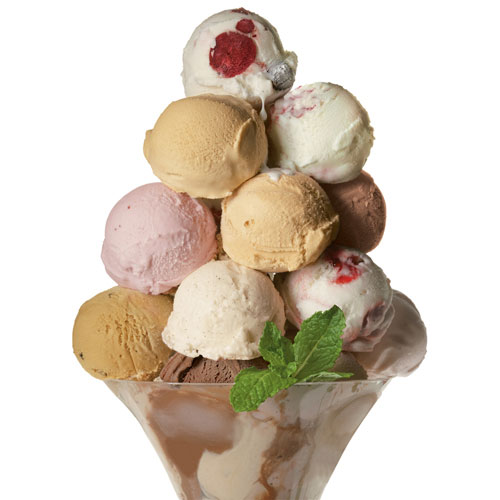
\includegraphics[scale=0.3]{ice_cream.jpg}

\end{titlepage}

\pagebreak

\tableofcontents

\pagebreak

%Disclaimer page

\section{Disclaimer}
This business plan has been prepared by SubZero Ice and is being provided to a limited number of persons, at their request.  This document is confidential and is only being made available to parties who agree to keep it confidential.  Neither this business plan nor any part of it shall be copied, reproduced or distributed to others at any time without the prior written consent of SubZero Ice. By accepting this document the recipient is deemed to undertake and warrant to SubZero Ice that the recipient will keep it confidential and that the recipient shall return all copies of this document to SubZero Ice immediately upon request.
Although SubZero Ice has taken reasonable care to ensure that the information contained in this document is accurate, no other representation or warranty, express or implied, is or will be given by SubZero Ice or any of its agents.  No responsibility is or will be accepted by SubZero Ice or any of its agents as to the accuracy or completeness of this document or the information or opinions contained herein.  Recipients must make their own investigations and must satisfy themselves as to the condition and prospects of SubZero Ice and the accuracy and completeness of statements contained herein.
Any financial projections given in this plan are illustrative only.  Because of the early stage nature of SubZero Ice’s business, none of the projections given in this document should be taken as guaranteed to be attainable, nor should they be taken as implying any indication, assurance or guarantee that those assumptions are correct or exhaustive.

%Tables
\begin{center}
  \begin{tabular}{ | l | c | }
    \hline
    Date Modified: & 10/03/2013 \\[2ex] \hline
    Document Version & V1.0 \\[2ex] \hline
    Author/Editor: & bmh10, cmn10, gl10, jbw10, mjs10, tg10 \\[2ex]
    \hline
  \end{tabular}
\end{center}

\newcolumntype{C}[1]{%
 >{\vbox to 5ex\bgroup\vfill\centering}%
 p{#1}%
 <{\egroup}}  

\begin{center}
\begin{tabular}{| C{3cm} | C{5cm} |} 
    \hline
    Issued to:     & ............................. \tabularnewline \hline
    Company:       & ............................. \tabularnewline \hline
    Date of issue: & ............................. \tabularnewline \hline
    Copy number:   & ............................. \tabularnewline \hline
  \end{tabular}
\end{center}

\pagebreak

%-------------------------------------------------------------------------------

\section{Executive summary}

SubZero Ice is an innovative business aimed at providing ice-cream in a more personal, novel and exciting way. Our patented process allows us to use liquid nitrogen as a freezing agent, providing customers with delicious, velvety smooth ice-cream along with a fantastic visual display as they watch their chosen ice-cream being prepared. What sets us apart from the competition is our focus on providing a unique customer experience as well as producing the highest quality ice-cream. In addition our instantly recognisable laboratory-themed stalls, patented process and enthusiastic ice-cream makers ensure that no one can pass us by unnoticed. We also pride ourselves on our use of fresh, organic ingredients in all of our products. \\

At the current time our main business focus is on acquiring a positive reputation at prestigious public events throughout the UK. During this period of growth and learning our business has recieved a remarkable amount of interest from some of the major event organisers in the UK as well as some press coverage. We have recieved hundreds of invitations to operate our stalls at public events, however given the relative age of our business coupled with our rapid success, we currently do not have the capital required to meet the demands of our expanding customer base. Having seen firsthand how customers react to our product we believe that it is time to take our relatively small business to the next level, hopefully expanding the area within which we operate to the whole of the UK. \\

Some of the companies that have already shown an interest in our business include the London Science Museum, Alton Towers, Odeon Cinemas, London Royal Parks and the organisers of music and arts festivals such as Glastonbury, Reading and Latitude. We have provided ice-cream and entertainment with much success at a large variety of events and demonstrations across England.


\section{Vision statement}

Our main goal is and always will be not only to provide great tasting ice-cream for our customers but also to provide them with an memorable experience. We strongly believe that their is a direct relationship between the amount of fun our staff are having and the number of customers we can attract. We also place the highest priority on producing quality ice-cream as we realise that even if the novelty of our product begins to fade over time, we will still be making the tastiest ice-cream on the market. \\

Our vision for the future is to revolutionise the ice-cream market through our introduction of liquid nitrogen to the production process. The technology and knowledge required to produce liquid nitrogen ice-cream has been around for some time now, however we believe that we are the first business in the UK to take advantage of the superior ice-cream which can be made through the use of this process. Having patented our unique process we believe that we are in a prime position to increase market standards and alter the way other businesses approach ice-cream production. \\

At SubZero Ice we place great importance on being ethical and economical within all spheres of business. All our stalls use solar panels to generate energy and our staff all follow a strict recycling policy which helps us to reduce costs as well as doing our bit for the environment. We also provide comprehensive training for all our ice-cream makers to ensure that they can safely handle liquid nitrogen in public. \\

Assuming that we manage to raise enough capital to expand our business activites over the next few years, we plan to focus our attention on scaling up our resources to match our ever increasing customer demand. At the same time we hope to branch out in other directions by introducing new products and also streamlining our specialised equipment which will allow our products to be introduced to establishments in the hospitality sector such as at bars and cafes. \\

\section{Market Analysis}
  
  Before delving into our business structure and our ideas for the future we though it would be wise to give a general overview of the current state of the ice-cream and conveniene foods markets so that the reader can gain a deeper insight into the current climate we are working in.

  \subsection{Market Drivers and Trends}

   We first take a look at current trends within the markets we are involved with and relate each observation to our own business. We hope that by predicting the direction the market is taking we will be able to meet and exceed our customer's expectations.
   
  \begin{itemize}
  \item The ice-cream market boasted a 9\% value growth in 2012, an improvement over the increase seen in 2011. It is believed that this increase is mainly due to good product innovation, large marketing campaigns and a renewed desire to purchase indulgance foods in the UK. The London Olymipics has also had a large impact on the ice-cream market with sales expected to top the £1bn mark for the first time in 2013. This has led us to believe that now would be a great time to expand our business to take advantage of this period of value growth in the market.

  \item It has been noted by several market experts that people do not seem to be holding back on purchasing culinary treats even during times of economic challenge. The ice-cream market has even seen growth during some of the hardest periods for the UK economy. It has been suggested that people are seeking comfort foods more often as a result of increased stress, leading to overall market growth.

  \item The use of liquid nitrogen in consumer food products is increasing as more businesses turn to  ``molecular gastronomy'' (the science of investigating and explaining how physical and chemical transformations can be made during cooking) in order to improve the taste and visual appeal of thier products. For example, some modern chefs use liquid nitrogen in the kitchen to change the consitancy of food. The cocktail industry have already taken note of this trend and have started to introduce products which use liquid nitrogen, mainly for its visual effect. We predict that in the future more companies will turn to molecular gastronomy in order to gain a competitive advantage. Since we have patented our unique ice-cream making process, which makes use of liquid nitrogen, we feel that we are in a strong position to take the majority market share for our niche in the market. 

  \item Events and hospitality companies are constantly looking to put on more of a show to gain an advantage over competitors and attract more people. Large festivals such as the main music festivals are attracting more people each year. We therefore intend to make it a priority to have stalls at these events as they will give us a lot of public exposure. We currently have a strong relationship with some of the major event mangers in the UK and we hope to solidify our partnership with them even more in the future.

  \item Historically successful ice-cream products are primarily those which have the most market appeal and capture the consumers imagination. With our product we hope to generate lots of consumer interest through our unique approach to ice-cream as it is generally accepted that innovation will be the main driver of growth over the next few years. Many ice-cream companies are expected to focus on developing new products, particularly in the premium segment, as indulgence remains a key consumer trend. We believe that our product will be able to satisfy this desire for innovation and quality seen at the current time, while also being more affordable than most of the premium brands on the market.

  \item In comparison to the ice-cream market, the frozen yoghurt market is relativaly underdeveloped and is therefore an area of opportunity. At SubZero Ice we have already begun researching how we can use our patented process to produce frozen yoghurts in the future.

  \end{itemize}


  \subsection{Market Segments}

  The ice-cream products currently on sale can be roughly segmented as the diagram below shows.
  %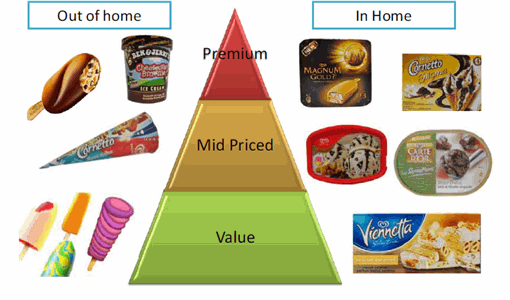
\includegraphics[scale=0.3]{pricepyramid.gif}

  Value ice-cream brands are the most common. The products in this segment are often fairly inexpensive and the companies that produce them rely on selling large quanties to make a significant profit, however they typically cost less to produce so the relative profit per unit sold may actually be higher. At the other end of the spectrum are premium brand ice-creams. The products in this segment typically cost much more the design, produce and package. Brands in the premium segment are typically marketed more heavily that value brands. However since the products are more luxurious, more can be charged for products in this category and hence the average transaction value is greater. Additionally ice-cream products can be segmented further into products which are designed to be eaten out of the home or in the home. Obviously brands which are designed for home consumption can sell their ice-cream in larger tubs. This usually means that the customer pays more in a single transaction and they also get more ice-cream for their money. Ice-creams which target outdoor consumption are usually not as good value for the customer, however they are essentially paying for the convenience of being able to buy a product which is prepacked in such a way that it is easy to eat.

  \subsection{The Opportunity for SubZero Ice}

  We strongly believe that there is a great opportunity for SubZero Ice given the market state and our current standing. We are at the forefront of our market niche and have already established ourselves as an exciting and innovative new brand. As already mentioned, premium brands are becoming increasingly popular in the UK. At SubZero Ice we intend to market our ice-cream as a premium brand in order to take advantage of this trend. However, since we are selling our ice-creams directly to the consumer, we can afford to spend more on making sure our ice-creams are the best tasting on the market since we do not have to spend as much on packaging and storing our ice-creams. Additionally we intend to do things a little differently from the majority of the market, by making ice-cream which not only tastes better than that of our competitors but is also delivered to the customer in a more exciting and personal way as we have seen in practice how well this works. \\


  \subsection{Target Markets}

  We aim to continue targeting large public events as this is what we do best. We have already signed long term contracts with some of the largest event managing companies in the UK. Given the visual appeal of our stalls and the lack of direct competition we are certain that public events will continue to yield large profits both financially and in terms of our reputation. \\

  In the future, and once we have raised enough capital, we plan to setup permenant shops in tourist areas around the UK. The advantage of this will be that we will not have to rely solely on public events which mostly take place in the summer months. We are also looking into the possibility of prepackaging some of our ice-creams to be sold from retailers rather than just from our stalls, though this is not currently our main focus. \\

  Interest in our stalls has also been expressed by various companies such as the London Science Museum and Odean cinemas. We are currently discussing long term solutions whereby we can have a stall inside their buildings. Since our stalls are more suited to outdoor use, we will need to consider other options if we are to accept these contracts. \\


\section{Products and Services We Offer}
  %Detail of what we are actually going to offer

  SubZero Ice offers customers a unqiue experience and ice-cream like no other on the market. We offer ice-cream made using our patented process which involves the use of liquid nitrogen as the freezing agent. Normally during the freezing process ice-cream is frozen relatively slowly meaning that the ice-cream contains large ice crystals. The advantage of using liquid nitrogen to freeze the ice-cream is that, due to the instantenous freezing, much smaller ice crystals are formed making the texture of the ice-cream much smoother and locking in more flavour. Through much research and experimentation we have come up with a process that produces perfect ice-cream everytime. \\

  Since our ice-creams are made infront of our customers we can also offer much more choice than other brands on the market. The customer can specify which fresh ingredients they would like including in their ice-cream. Given that we stock around 15 different ingredients at our stalls, the combinations are almost endless.This also means that we can cater for all personal preferences as our customers can choose how healthy or luxurious they would like their ice-cream to be. The majority of our fresh ingredients are fairtrade and organic as we believe that in order to make the best ice-cream we need to use the best ingredients. \\

  As well as offering the tastiest ice-cream on the market we aim to provide entertainment to all of our customers. As mentioned the use of liquid nitrogen is the secret to making our ice-cream so delicious, however it also creates a great visual spectacle. Additionally our stalls are specifically designed to fit in with the scientific nature of our ice-cream production. The stalls are designed to look like laboratories, with numerous test tubes and flasks filled with colourful liquids along the front of the stalls. Our staff also dress in lab coats and goggles to add to the themed experience we want to create. Due to our focus on creating highly visual stalls we usually find that we manage to attract many more interested customers than similar convinience food stalls nearby. \\
  
  In terms of future products we are already experimenting with using variations of our patented process in order to produce frozen yoghurt products. The frozen yoghurt market is very underdeveloped compared to the ice-cream market so we feel that it will be benifical to expand our product range to include them. Longer term we hope to introduce some of our products, perhaps prepacked, into the mainstream ice-cream market to be sold by retailers. We are also looking at the possibility of modifying our equipment so that is can be used in permenant shops. \\


\section{Business Model \& Structure}
  %How the business will actually work

  SubZero Ice is a workers' cooperative meaning that all of our members can have a say on any decisions which need to be made and they all have a fair stake in the business. At SubZero Ice we are guided by the cooperative values of self-responsibility, democracy, equality, equity and solidarity. We also place great importance on following the ethical values of openness, honesty and social responsibility. We aim to provide a fair and empowering environment where everyone, and no-one, is the boss. In many traditional businesses the workers are simply part of the company machinary and it is often the case that the people making big decisions are not the ones doing the groundwork. However at SubZero Ice we understand the importance and value of our members which is reflected in our fair pay and business structure based on equality. This structure has helped us to create a workforce who intrinsically care about the business and its future. Our benchmark for success is not only financial growth but also ensuring that we remain a democratic workplace which is rewarding to work in. \\

  When it comes to defending our choice to be a workers' cooperative when so many other firms are still choosing more traditional structures we simply refer to the statistics. The failure rate amongst co-ops if extremely low compared to the 80\% of traditional business startups which fail during the first few years. We believe that this is due to the much greater support available within co-op communities, the help given by other cooperative firms and the greater commmitment workers show when they know they can make a difference. \\

  A common question we get asked is how we can make decisions within our business structure when there are no leaders. For small decisions we usually use a voting system whereby each person the decision concerns has one vote and the majority view is held to be in the best interests of the company. However for larger decisions or if the vote is very close then we use consensus decision making. This involves asking people questions individually and taking note of their responses so that we can build up a picture of all the hidden issues and motives behind people's decisions. We continue to do this until a solution which everyone can support is arrived at. This has proved to be a better way of making big decisions as unlike the voting system it is impossible to ignore the minorities who are unhappy. With this scheme we usually find that we can create a win-win solution that amalgamates everyone's best ideas. It also means that we hardly ever have to go back and revisit old issues once a decision has been made. \\

  Currently our business is split into six teams with each team focussing on a specific area. Each team has a small group of people within it who are responsible for communicating decisions or developments of importance to the other teams. Below we list the six teams and summarise their role in the business.
  \begin{itemize}

  \item Design and Innovation Team - responsible for generating and researching new product ideas, as well as constanly reassessing what can be improved with our current range of products.

  \item Marketing and Public Relations - responsible for creating public interest in our brand, dealing with client queries and keeping our website up to date.

  \item Finance - responsible for budgeting, planning for the future and overseeing the finances of the business.

  \item Ice-cream Makers - responisible for selling ice-cream from stalls at events and putting on a show for customers.

  \item Transport - responsible for transporting equipment to and from events and ensuring all equipment is safely stored in our storage depots.
  
  \end{itemize}


  \subsection{Suppliers \& Distribution}

  We have a good relationship with all of our current suppliers. Below we list our suppliers and what they provide for us.

  \begin{itemize}
  \item Mansfield Cryogenics - offer us a complete liquid nitrogen delivery service with quantities from 300ml to 500 litres capable of being delivered anywhere within the UK. They provide some of the most competitive pricing in the industry as they deliver on a scheduled cyclic basis meaning they can make several deliveries together to cut costs. More information can be found on their website at http://mansfieldcryogenics.com/

  \item Reynolds - supply us with the fresh fruit we require to make our ice-creams. They are one of the UKs leading fresh fruit distributors and are suppliers of more than 1,000 different types of fruit and vegetable from around the world. More information can be found on their website at http://www.reynolds-cs.com/

  \item Freshways - supply us with milk and natural yoghurts which we use to make our ice-creams. They offer us reduced rates since we make orders regurarly. More information can be found on their website at http://www.freshways.co.uk/

  \item HB Ingredients - supply us with chocolate and other sweet ingredients we use in our ice-creams. They are the largest independent chocolate distributor in the UK and offer a discount for businesses who order in bulk. More information can be found on their website at http://www.hbingredients.co.uk/

  \item D.P. Structures Ltd - provide bespoke market stall construction services and are based in Burnley. They offer a complete service from inital designs and concept drawing, through to fabrication, construction and installation. More information can be found on their website at\\
   http://www.dpstructures.co.uk/structures/market-buildings/

  In terms of our distribution model we have to ensure that we have enough ingredients and liquid nitrogen to cover our requirements at all times and that they are ready to be used on the day of an event. The transport team as well a being responsible form transporting equipment to events, as mentioned above, are also responsible for ensuring that stalls are stocked with everything they need to be operational. At the end of an event the transport team are also responsible for recording how much liquid nitrogen and ingredients are left over. We keep track of these statistics for each event we are contracted at so that we can analyse where we could be saving money in the long term.
  \end{itemize}

  \subsection{Current Equity Structure}

  \subsection{Technical Expertise}

  Since we are a cooperative company we do not have a management team, however there are certain people within our company who we could not function without.
  Below we list the people who act as role models within the company and have helped us to attain our current level of success.

  {\bf Tim Gates - Founder \& Director} \\
  Tim has over 15 years experience working within the convenience foods industry. Having previously worked for Unilever, he knows what it takes to make a business succeed. He is dedicated to creating a business in which everyone is treated fairly and with respect. From previous experience he has see how the culture within a company can easily become polluted with unfairness and mediocrity given the wrong people or business structure. Tim sees himself not as the CEO of the company but as a critical observer with the best interests of everyone at heart.

  {\bf Ben Homer - Chair \& Company Advisor} \\
  It is Ben's job to ensure that as a company we are standing by our cooperative and democratic ideals. Ben's rather untraditional role helps to ensure that we stand by our aims to include everyone in decision making and to treat everyone as equal. Ben oversees important company meetings to ensure that all views are taken into account. He also deals with any issues which arise regarding company structure or employee dissatisfaction. Ben has plenty of previous experience working within cooperative businesses and is often able to give the company advise on how to avoid pitfalls common to cooperative enterprises. Ben is also responsible for nurturing our unique business culture by planning team building events or lunch time activites at our London office.

  {\bf Jon Watson - Secretary} \\
  Jon is responsible for dealing with the paperwork at meetings, keeping track of our accounts, annual legal reporting and membership lists. Having worked as a secretary for many years Jon has proved to be a great motivator and encourager within meetings. His focussed attitude and personable nature make him a much respected member of the company.

  {\bf Martin Sidery - Treasurer} \\
  Having previously worked in the finance district in London, Martin realised the need for a change. Since then he has been helping our finance and planning team to put our money to best use. Martin is an expert in financial planning and is extremely willing to share his wisdom and experience with the rest of our finance team.
 
  {\bf Conor Nevin - Product Design \& Innovation} \\
  Conor has a highly varied background in product design having previously having worked on successful projects in the technology, games and food industries. With his vast array of experience and supreme attention to detail Connor acts as a mentor to our product design team. He often encourages our designers to think laterally when coming up with new product ideas. His quiet motivation and ability to see the potential in every idea make him an invaluable asset to the company.

  {\bf Graham Lyon - Marketing and Public Relations} \\
  Graham has worked in marketing since he left university and has racked up an astonishing amount of experience within a multitude of different market sectors. His self deprecating and jovial manner often hide his marketing genius, however the huge amount of interest he has managed to generate in the company within such a short period of time speaks for itself.


\section{Competition}

  Unilever UK Ltd is currently the leading business in the ice-cream market, with a 30\% market share in 2012. The company's retail sales saw a 22\% increase during the same year, indicating the level of growth the market is currently going through. Unilevers most popular brands are Magnum and Cornetto. They are also the global business operators of Ben \& Jerry's, Cart D'Or and Walls. The company continues to offer new varients on existing products which have all been well recieved by the public. Recently they have also been spending large amounts on advertising which has also increased their success. For example the release of Ben \& Jerry's Core range was supported by a huge £5 million advertising campaign. R\&R Ice Cream are the other notable market leader, owning brands such as Nestle, Ribena, Kelly's of Cornwall and Thorntons. \\

  Considering the domination of the mainstream ice-cream market by the leading companies we have chosen to focus on our market niche which is supplying ice-creams at large events. Within this sector there are very few direct competitors and certainly none with the success and interest that we have already generated. We believe that we provide a better, more scalable product than our direct competitors and are therefore in prime position to take the majority of the market share within our niche. Having said this we realise the effect the market leaders are having on the habits of consumers which is why, if we are to continue to be succesful, we will need to stay one step ahead of the market and continue to be innovative in our product design.

\subsection{Competitive Advantages}

We believe our product has several clear competitive advantages over other ice-cream brands currently on the market. Below we list some of these advantages.

  \begin{itemize}
  \item Our ice-cream is velvety smooth, creamy and freshly made. Due to the unique freezing process our ice-cream is guaranteed to be free of large ice crystals giving a delicious texture like no other ice-cream on the market.

  \item Our process instantly freezes the freshest of ingredients, providing an unsurpassed flavour. Since we make the ice-creams freshly for our customers it means there is also much more scope for different flavourings. Customers can choose any of our fresh ingredients they like and combine them in any way they choose.

  \item Another clear competitive advantage of using liquid nitrogen is that it provides a unique and fascinating spectacle that normal ice cream stalls simply cannot provide. We believe that creating an impressive visual experience for our customers and putting on a show is almost as important as the ice-cream itself.Through this unique blend of entertainment and delicious ice-cream we hope to capture the imaginations of our customers.

  \item We also have the advantage of novelty. Many consumers will never have tried or even heard of liquid nitrogen ice-cream before and so we hope that one-off novelty purchases will help us to be even more successful, especially during the first few years of business.

  \item Since the customer has complete control over the ingredients which are used in their ice-cream, apart from the base ingredients, our ice-creams have the potential to be more healthy than our competitors. This can only help, given the current trend towards healthy, low-fat foods.
  \end{itemize}

\section{Intellectual Property Assets}

  \subsection{Patents}

  We have patented our unique ice-cream making process which involves the use of liquid nitrogen and various other secret ingredients. In terms of technology we currently use standard liquid nitrogen storage tanks at our stalls which have been customised to fit in with our stores' theme. Our innovation is not in the technology or ingredients we use themselves but in how we use them in conjuncation to create the best tasting ice-cream on the market.

  \subsection{Future Intellectual Property Development}

  We are currently researching how we can use liquid nitrogen to make frozen yoghurt as we believe this is an untapped market. We plan to patent this once our research is finished. Additionally we hope to raise enough capital to be able to purchase more compact storage units, in order to branch out our business into cafe's or bars.


\section{Business Development Plan}




  % summary of detailed plan including
  % prioritisation
  % validation
  % offers
  % routes to market

  \subsection{Current Situation \& Resources}

  Currently have sold ... and have established technology

Currently have capability to operate … stalls

  \subsection{Longterm \& Shorterm Goals}

    Shorterm goals

    Maximise number of sales and expand business using money from investors

    objective - maximise sales -> how

    Longterm goals

    Design new products - specifically forzen yoghurt products
    Prepackaged ice-cream products

  \subsection{Sales process}

  \subsection{Target customers}
Tourists of all ages. Especially families with children and young adults
who are more likely to be at festivals.

 - Want to move away from small temporary stalls to more permanent
installations

 - Want to target large customers in the hospitality sector

 - Odeon, Alton Towers, Thorpe Park?

   LTV = (Tn + ATV + LT) - (CoA + CoR)
       = (no + average transaction value + lifetime value) - (cost of aquisition + cost of retention) 

  \subsection{Current key customers}

  Currently provided product as one off temporary stall for 

  They have expressed interest in returning to us

  \subsection{Marketing, PR and Communications}
  At the moment our main form of marketing are the stalls themselves. Given the exciting way we present our product the stalls often generate a lot interest, which large groups of people watching our ice-cream being made simply out of interest before they make a purchase.

  In the future as we expand and move into more permanent fixtures we hope to use more traditional marketing methods.

  We are currently developing a website which we think will play a vital role in generating more consumer interest. Through this website we will give our customers the opportunity to contact us and leave feedback on their experience with our product.

  We also wish to focus strongly on interacting with social media sites such as Facebook and Twitter as we believe this will allow us to quickly generate interest, receive comments and interact directly with our customers. Additionally this will allow us to collect information about our customers, for example the average age of our customers. It is with such information that we hope to be able to tailor our future marketing.

  In order to generate interest online we will hold regular competitions and prize draws, in which the winners will receive vouchers to spend on our ice-cream. We also plan to video some of our stalls in action and post on YouTube.???

  \subsection{Staff Recuritment}

  We are highly aware of the fact that the success of our business depends on the people involved in it. Since we are a worker's cooperative, choosing the right mix of people is even more important as we all have to work together as equals and share responsibility for the business. When recruiting new staff we first of all consider whether they have similar values to our exisiting members, as we realise that in order to be successful our members must be able to work together as a commited unit, all moving towards the same ideals or reaching compromises where necessary. We also ensure that all new members are commited to working in a cooperative environment, that they know what to expect and that they will be able to handle the responsibility placed on them. Additionally we ensure that potential members are self-motivated, can show initiative and have the practical skills required for their chosen role.

  All new members will be assigned a personal mentor during their first month to ensure that they are fitting into the company and know what is expected of them. We also carry our ongoing reviews to ensure that our members are the right people for the job and they are working well together, which requires a lot of honesty from all members of our business.

  As our customer base contniues to expand we will need to recruit the following staff:

 {\bf Ice-cream Makers} - ice-cream makers are the life and soul of SubZero Ice. In order to qualify for the role candidates will have to show genuine enthusiasm and commitment to the company as well as being able to work well under pressure infront of crowds. Candidates must also be very flexible as they will have to travel to different locations each day if not working at a fixed stall. All ice-cream makers will receive suitable training and must pass a health and safety test to ensure they can safely handle liquid nitrogen and that they understand the risks of using liquid nitrogen on a daily basis. Perks include free entry to large festivals, free ice-cream and the opportunity to have fun at work.

 {\bf Marketing and PR Staff} - our marketing staff have the huge responsibility of creating relationships with potential clients (event managers) and generating public interest in our unique brand and products. They have the opportunity to shape our future and maximise our success. In order too qualify candidates must have a flair for marketing, be able to listen to the ideas of others and give constructive feedback. Some members of the PR staff will also be responsible for managing our online prescence by replying to customers, making note of customer feedback and creating competitions and prize-draws for customers.

{\bf Product Designers} - our product designers must realise what our customers want before they want it. In order to qualify for this role candidates must have worked with at least one previous product design team and be able to think laterally. Product designers work with our current brand and public image to create new and exciting products. At SubZero Ice we are not scared of change and so we also encourage our product designers to be innovative by having weekly meetings in which adventourous theories or experimental product ideas can be discussed and shared.

{\bf Transport Team} - our transport team are responsible for moving our stalls and equipment to events and setting them up. They are also responsible for taking all equipment back to our nearest storage hold after it has been used. All candidates must have a full UK driving license and will be given relevant health and safety training on starting. Members of the transport team must be flexible as they will have different working hours depending on which events we are currently operating at. They may also have to transport our equipment from one storage depot to another when we require more equipment in a certain area of the country.

 {\bf Finance Team} - our finance team are responsible for assessing our current finances, analysing what could be done better and producing financial projections. All canditates must have a strong mathematical background and the desire to make a positive difference to our company. As a business we do not want to rely on gut feelings as to what is optimal for our business but on real world data and mathematical models. Our finance team are therefore responsible for deciding how we should balance our spending as a company in order to increase our profit and the overall value of SubZero Ice.

 {\bf Legal Team} - we will require a small team of specialised legal associates who can advise us on legal matters especially as our business grows and we receive more clients. Although members of the legal team will technically be external to the company, they will all be granted membership of the business cooperative and hence will be able to buy and sell shares within the company.

 {\bf Voluntary Staff \& Students} - we are also looking for voluntary staff to help with the day to day running of SubZero Ice. We are currently in process of organising an internship and summer placement scheme for students. We feel that SubZero Ice has a lot to offer volunteers and our cooperative working environement ensures that our volunteers are respected and treated as equals by our staff.


  \subsection{Facilities}

  Currently all of our staff operate from our headquarters in central London.
  We already own a small office in central London from which we operate.
  Will need large office as number of staff increases.

  Currently store equipment in a storage warehouse when not in use.
  Will need new storage locations around the country to make access to equipment easier.


\section{Financial Plan \& Funding}

\subsection{Financial History \& Startup Costs}

Below are diagrams which show our initial start up costs from about 6 months ago.

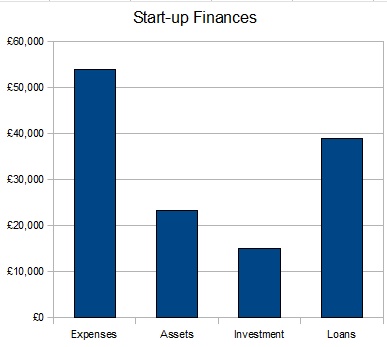
\includegraphics[scale=1.0]{startupFinance.png}
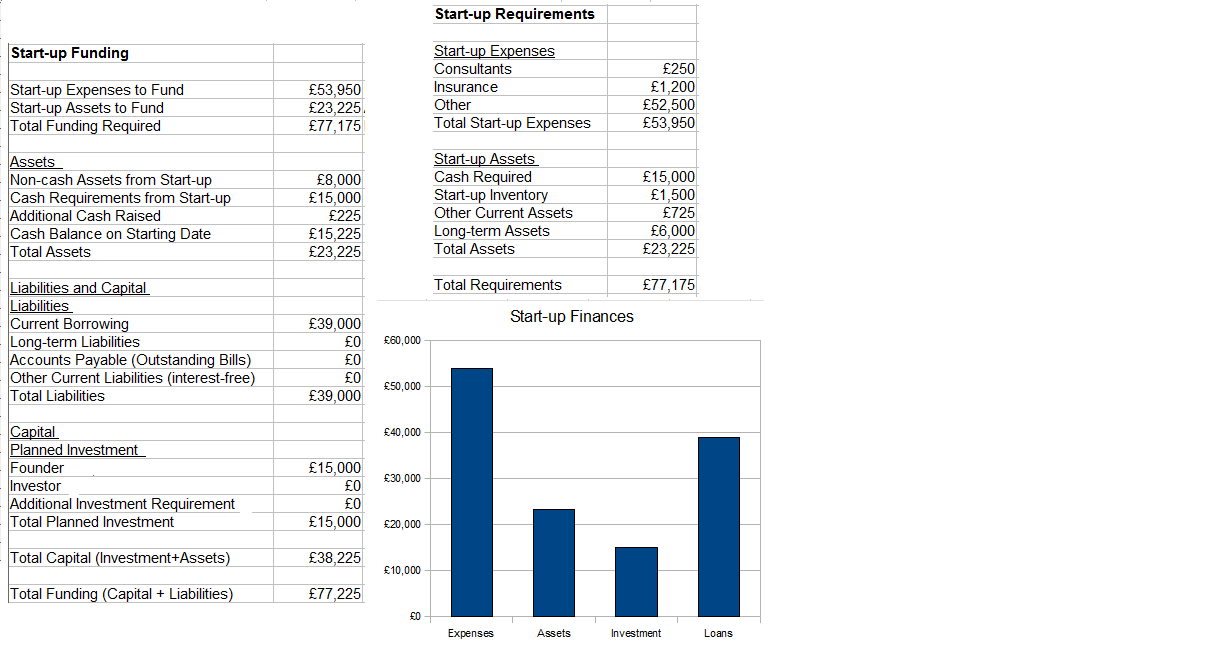
\includegraphics[scale=1.0]{startupFinanceData.png}

Below our finance summary for the first six months of business is shown.

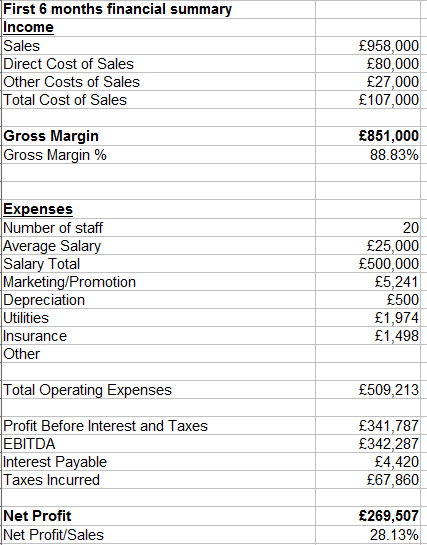
\includegraphics[scale=1.0]{firstSixMonths.png}

\subsection{Pricing Strategy}

We plan to continue selling our ice-cream with the following pricing strategy.

1 scoop £2.25
2 scoops £3.85
3 scoops £4.65
Additional scoops +£1.00
Extra toppings £0.30 each

\subsection{Projected Profit and Loss}

\subsubsection{Pro Forma Profit and Loss}

\subsection{Projected Cashflow}

\subsubsection{Pro Forma Cashflow}

\subsection{Raising Capital}



Last year financial summary

Income
 - total sales       
 - grants/donations
 - interest from invested money

 Total income

 Expenditure
 - wages and salaries - 60 staff * £25 000
 - training - £50 000
 - rent, phone bills, utilities £10 000
 - advertising £20 000
 - taxes such as VAT, corporation tax and business rates
 - legal and professional fees £3 000
 - buying equipment and ingredients 
 - repairs and maintenance £2 000
 - working capital 
 - loan repayment

 Total expenditure = 

Our members have decided on the course of action which needs to be taken financially in order for us to meet our goals.

We are looking to raise £5 million in captial, to allow us to expand our business and develop our range of products.

Main costs:
 - Stalls - LN2 tanks + supply - 50 litre liquid nitrogen tanks – around £1000 and Each litre of liquid nitrogen costs around £1.25
 - Transport vechicles
 - Storage space
 - Staff recruitment and wages
 - New London HQ - expand existing offices - £0.5 million
 - Ice cream ingredients
 - Marketing and website




Each litre of ice-cream requires...

Office and storage space in London will cost

Ideally we would like the capital to be able to purchase equipment to
produce our own liquid nitrogen from the air.(???)

Use of Funds

More stalls

More marketing needed

Need to grow beyond London

Professional website and web prescence on social media sites


SHARES

Revenue from sales in the previous year was around £3.5 million. (total income without subtracting any expenses) 
Gross profit of £2.9 million (difference between sales and cost of sales i.e. revenue - cost of goods)
Net profit of £1.8 million (actual profit when all expenses are subtracted)

%Graph to show financial growth over first year of business


revenue
 - retail
   licence
   other sales

profit/net income
 - gross
   net
   EBITDA
   NPV

costs
 ...

\section{Risk Analysis \& Exit Strategy}

Little risk as we are already an established business, struggling to keep up with customer demands.

If market changes rapidly. Look at options available to us. Other market segments we can move into.



\section{Corportate Information \& Contact Details}

Address: \\

SubZero Ice
Level 2-3 
Langley House
Langley Ln
Vauxhall
London
SW8 1GB

Contacts: \\

Public Relations \& Enquiries: 07856054971 | enquiries@subzeroice.coop


\end{document}


\section{Company History}

SubZero Ice started with a group of friends who had a love for ice-cream and a desire to remove themselves from underpaid jobs in which they had no control. Together they wanted to create a revolutionary ice-cream business that used science as a means to produce the best ice-cream on the market. The company recieved much unexpected interest from large event organisers who were looking to hire innovitive new consumer goods stalls at their events. Soon after SubZero Ice was born. Having started off small the team and business quickly grew, recieving attention from the media and large music festival organisers, with their first major contract being with the organisers of Glastonbury Festival. Since then the company has continued to grow and recieve contract offers from other large firms including Odean Cinemas and London Royal Parks.

\section{Apendix A - References}

http://www.radicalroutes.org.uk/publicdownloads/setupaworkerscoop-lowres.pdf - For useful information on everything to do with workers' cooperative businesses.
